\documentclass[12pt,tightenlines,letterpaper]{scrartcl}
\usepackage{lmodern}
\usepackage{ifxetex,ifluatex}
\usepackage{fixltx2e} % provides \textsubscript
\ifnum 0\ifxetex 1\fi\ifluatex 1\fi=0 % if pdftex
  \usepackage[T1]{fontenc}
  \usepackage[utf8]{inputenc}
\else % if luatex or xelatex
  \ifxetex
    \usepackage{mathspec}
  \else
    \usepackage{fontspec}
  \fi
  \defaultfontfeatures{Ligatures=TeX,Scale=MatchLowercase}
\fi

%%% Needed to write listtodonotes, and listofalgorithms, but the problem is listoftodonotes
 \usepackage{morewrites}
\usepackage[
HomeHTMLFilename=index,     % Filename of the homepage.
%HTMLFilename={node-},       % Filename prefix of other pages.
%IndexLanguage=english,      % Language for xindy index, glossary.
latexmk,                    % Use latexmk to compile.
%   OSWindows,                  % Force Windows. (Usually automatic.)
mathjax,                    % Use MathJax to display math.
]{lwarp}


\title{Block Chain Notes}
\author{David Li}
\setcounter{tocdepth}{2} % Include subsections in the \TOC.
\setcounter{secnumdepth}{2} % Number down to subsections.
\setcounter{FileDepth}{0} % Split \HTML\ files at sections, in this case chapters?, 0 for chapters?
\booltrue{CombineHigherDepths} % Combine parts/chapters/sections
\setcounter{SideTOCDepth}{1} % Include subsections in the side\TOC
\HTMLAuthor{David Li} % Sets the HTML meta author tag.
\HTMLLanguage{en-US} % Sets the HTML meta language.
\HTMLDescription{A list of cheatsheets for courses at the University of Victoria}% Sets the HTML meta description.
\HTMLFirstPageTop{ CheatSheets \fbox{\includegraphics[width=1\linewidth]{Images/Ethereum-Cover.png}}}
\HTMLPageTop{\fbox{\includegraphics[width=1\linewidth]{Images/Ethereum-Cover.png}}}
\HTMLPageBottom{Made by David Li}
\newcommand{\printTitle}{Insert a title Here} 
\usepackage{graphicx} % Required for including pictures
\graphicspath{{Images/}} % Specifies the directory where pictures are stored

%%%% Useful Packages loaded without much configuration %%%%%%
\usepackage[margin=2.54 cm]{geometry} % Set dimensions for page layout
\usepackage{kpfonts}	    % Fonts used in the title page
\usepackage{eso-pic}        % Background pictures in the title page
\usepackage[many]{tcolorbox}		% Fancy Math equations	
\usepackage{tabularx}		% Tabulars with adjustable-width columns

%\usepackage{makecell,tabularx}
\newcolumntype{L}{>{\raggedright\arraybackslash}X}

\tcbuselibrary{skins} 	% used with tcolorbox 
\usepackage{transparent}	% Create transparent background images
\usepackage{lipsum}  % Garbage text
\usepackage{url}	 % links to websites
\usepackage{pdfpages} % to include pdf pages
\usepackage{booktabs}	% Make high quality tables
\usepackage{colortbl}	% Color tables
\usepackage{xfrac}		% Make fractions nice in tables
\usepackage{enumitem}	% itemize, enumerate
\usepackage{array}
\usepackage{setspace}   % double spacing as required in UVIC co-op reports
\usepackage{titlesec} % Select alternative section titles
\titlespacing*{\section}
{0pt}{5.5ex plus 1ex minus .2ex}{4.3ex plus .2ex}	% Not sure about this spacing
\usepackage{multirow} % Create tabular cells spanning multiple rows.

%CHANGE Link colours as needed
\definecolor{linkColor}{HTML}{453737}	

\usepackage{hyperref}	% Create links in document
\hypersetup{linktocpage}	% Allow clickable links
\hypersetup{
    bookmarks=true,         % show bookmarks bar?
    unicode=false,          % non-Latin characters in Acrobat’s bookmarks
    pdftoolbar=true,        % show Acrobat’s toolbar?
    pdfmenubar=true,        % show Acrobat’s menu?
    pdffitwindow=false,     % window fit to page when opened
    pdfstartview={FitH},    % fits the width of the page to the window
    pdftitle={Work Term Report},    % title
    pdfauthor={David Li},     % author	
    %linktoc=all,     %set to all if you want both sections and subsections linked
	colorlinks   = true, %Colours links instead of ugly boxes
	urlcolor     = blue, %Colour for external hyperlinks
	linkcolor    = red, %Colour of internal links
	citecolor   = green %Colour of citations
}


\usepackage{float}    % used for float­ing ob­jects such as fig­ures and ta­bles.
\usepackage{caption}
%\captionsetup[figure]{labelfont=sf,textfont={sf}}
%\captionsetup[table]{labelfont=sf,textfont={sf}}
% \usepackage{parskip} % no indents, don't use in lwarp
\usepackage{tikz}	 % for drawings and cool graphics

%% Math packages %%
\usepackage{siunitx}	% SI units
\usepackage{mathtools}	% LOAD MATH
\usepackage{amssymb}  	% MATH Symbols


%%%%%%%%%% COLORS %%%%%%%%%%%%%%%%%%%%%%%%%%%%%
\definecolor{titlepagecolor}{cmyk}{1,.60,0,.40}

%%%%%%%%%%%%%%%%%%%%%%%%%%%%%%%%%%%%%%%%%%%%%%%%%%%%%%%%%%%%%%%%%%%%%%
%%%%%%%%%%%%%%%%%%%%%%%%%%%% CODE STYLINGS %%%%%%%%%%%%%%%%%
%%%%%%%%%%%%%%%%%%%%%%%%%%%%%%%%%%%%%%%%%%%%%%%%%%%%%%%%%%%%%%%%%%%%%%%%

\usepackage{listings} % For source code
\DeclareCaptionFont{white}{\color{white}}
\DeclareCaptionFormat{listing}{\colorbox{titlepagecolor}{\parbox{1\textwidth}{#1#2 \quad #3}}}
\captionsetup[lstlisting]{format=listing,labelfont=white,textfont={white,sf}} % for fancy boxes

\lstdefinestyle{default}{frame=tb,
	aboveskip=3mm,
	backgroundcolor=\color{cornsilk},
	belowskip=3mm,
	showstringspaces=false,
	columns=flexible,
	basicstyle={\ttfamily},
	numbers=none,
	numberstyle=\tiny\color{red},
	keywordstyle=\color{blue},
	commentstyle=\color{green},
	stringstyle=\color{purple},
	morekeywords={fclose, exit, printf, fscanf, strcpy, strlen,
		strcmp, fprintf},
	breaklines=true,
	breakatwhitespace=true,
	tabsize=3,
	captionpos=t,
	columns=flexible,
}

\definecolor{verylightgray}{rgb}{.97,.97,.97}

\lstdefinelanguage{Solidity}{
	keywords=[1]{anonymous, assembly, assert, balance, break, call, callcode, case, catch, class, constant, continue, contract, debugger, default, delegatecall, delete, do, else, event, export, external, false, finally, for, function, gas, if, implements, import, in, indexed, instanceof, interface, internal, is, length, library, log0, log1, log2, log3, log4, memory, modifier, new, payable, pragma, private, protected, public, pure, push, require, return, returns, revert, selfdestruct, send, storage, struct, suicide, super, switch, then, this, throw, transfer, true, try, typeof, using, value, view, while, with, addmod, ecrecover, keccak256, mulmod, ripemd160, sha256, sha3}, % generic keywords including crypto operations
	keywordstyle=[1]\color{blue}\bfseries,
	keywords=[2]{address, bool, byte, bytes, bytes1, bytes2, bytes3, bytes4, bytes5, bytes6, bytes7, bytes8, bytes9, bytes10, bytes11, bytes12, bytes13, bytes14, bytes15, bytes16, bytes17, bytes18, bytes19, bytes20, bytes21, bytes22, bytes23, bytes24, bytes25, bytes26, bytes27, bytes28, bytes29, bytes30, bytes31, bytes32, enum, int, int8, int16, int24, int32, int40, int48, int56, int64, int72, int80, int88, int96, int104, int112, int120, int128, int136, int144, int152, int160, int168, int176, int184, int192, int200, int208, int216, int224, int232, int240, int248, int256, mapping, string, uint, uint8, uint16, uint24, uint32, uint40, uint48, uint56, uint64, uint72, uint80, uint88, uint96, uint104, uint112, uint120, uint128, uint136, uint144, uint152, uint160, uint168, uint176, uint184, uint192, uint200, uint208, uint216, uint224, uint232, uint240, uint248, uint256, var, void, ether, finney, szabo, wei, days, hours, minutes, seconds, weeks, years},	% types; money and time units
	keywordstyle=[2]\color{teal}\bfseries,
	keywords=[3]{block, blockhash, coinbase, difficulty, gaslimit, number, timestamp, msg, data, gas, sender, sig, value, now, tx, gasprice, origin},	% environment variables
	keywordstyle=[3]\color{violet}\bfseries,
	identifierstyle=\color{black},
	sensitive=false,
	comment=[l]{//},
	morecomment=[s]{/*}{*/},
	commentstyle=\color{gray}\ttfamily,
	stringstyle=\color{red}\ttfamily,
	morestring=[b]',
	morestring=[b]"
}

\lstset{
	language=Solidity,
	backgroundcolor=\color{verylightgray},
	extendedchars=true,
	basicstyle=\footnotesize\ttfamily,
	showstringspaces=false,
	showspaces=false,
%	numbers=left,
%	numberstyle=\footnotesize,
%	numbersep=9pt,
	tabsize=2,
	breaklines=true,
	showtabs=false,
	captionpos=t
}
%%%%%%%%%%%%%%%%%%%%%%%%%%%%%%%
%%%%%% SQL style setup %%%%%%%%
\makeatletter
\newcommand{\lstuppercase}{\uppercase\expandafter{\expandafter\lst@token
		\expandafter{\the\lst@token}}}	%%%UPPERCASE SQL%%%%
\newcommand{\lstlowercase}{\lowercase\expandafter{\expandafter\lst@token
		\expandafter{\the\lst@token}}} %%% REGULAR CASE %%%%
\makeatother

\definecolor{mauve}{rgb}{0.58,0,0.82}
\lstdefinestyle{Oracle}{basicstyle=\ttfamily,
	keywordstyle=\lstuppercase,
	backgroundcolor=\color{cornsilk},
	emphstyle=\itshape,
	showstringspaces=false,
	morekeywords={ACCESS, MOD, NLS_DATE_FORMAT, NVL, REPLACE, SYSDATE,
		TO_CHAR, TO_NUMBER, TRUNC},
	numberstyle=\tiny\color{black},
	keywordstyle=\color{red},
	commentstyle=\color{green},
	stringstyle=\color{mauve},
	columns=flexible,
}
%%%%%%%%%%%%%%%%%%%%%%%%%%%%%%%%%%%%%%%%%%%%%%%%
%%%%%%%%%%%%%%%%%%%%%JAVA %%%%%%%%%%%%%%%%%%%%%%
\definecolor{javared}{rgb}{0.6,0,0} % for strings
\definecolor{javagreen}{rgb}{0.25,0.5,0.35} % comments
\definecolor{javapurple}{rgb}{0.5,0,0.35} % keywords
\definecolor{javadocblue}{rgb}{0.25,0.35,0.75} % javadoc
\lstdefinestyle{myJava}{frame=tb,
	basicstyle=\ttfamily,
	backgroundcolor=\color{cornsilk},
	keywordstyle=\color{javapurple}\bfseries,
	stringstyle=\color{javared},
	commentstyle=\color{javagreen},
	morecomment=[s][\color{javadocblue}]{/**}{*/},	% Make comments blue
	morecomment=[is]{/*}{*/},  % Remove comments
	stepnumber=2,
	numbers=left,    % print line numbers
	numbersep=10pt,
	tabsize=4,
	showspaces=false,
	showstringspaces=false,
	linewidth=\textwidth,
	columns=flexible,			% Important for keeping text in the frame
	breaklines=true,
}

%%%%%%%%%%%%%%%%%% ENDJAVA %%%%%%%%%%%%%%%%%%%%%
%%%%%%%%%%%%%%%%%%%%%%%%%%%%%%%%%%%%%%%%%%%%%%%%

%%%%%%%%%%%%%%%%%%%%%%%%%%%%%%%%%%%%%%%%%%%%%%%%%%
%%%%%%%%%%%%%%%%%%%%% JAVASCRIPT%%%%%%%%%%%%%%%%%%%
\lstdefinelanguage{JavaScript}{frame=tb,
	keywords={typeof, new, true, false, catch, function, return, null, catch, switch, var, if, in, while, do, else, case, break},
	keywordstyle=\color{blue}\bfseries,
	ndkeywords={class, export, boolean, throw, implements, import, this},
	ndkeywordstyle=\color{darkgray}\bfseries,
	identifierstyle=\color{black},
	sensitive=false,
	comment=[l]{//},
	morecomment=[s]{/*}{*/},
	commentstyle=\color{purple}\ttfamily,
	stringstyle=\color{red}\ttfamily,
	morestring=[b]',
	morestring=[b]"
}
\definecolor{cornsilk}{rgb}{1.0, 0.97, 0.86}
\lstdefinestyle{myJavaScript}{
	language=JavaScript,
	backgroundcolor=\color{cornsilk},
	extendedchars=true,
	basicstyle=\ttfamily,
	showstringspaces=false,
	showspaces=false,
	tabsize=2,
	breaklines=true,
	showtabs=false,
	captionpos=t,
}
%%%%%%%%%%%%%%%%%%%%%%%%%%%%%%%%%%%%%%%%%%%%%%%%%%
%%%%%%%%%%%%%% END CODE STYLINGS %%%%%%%%%%%%%%%%%
%%%%%%%%%%%%%%%%%%%%%%%%%%%%%%%%%%%%%%%%%%%%%%%%%

%%%%%%%%%%%%%%%%%%%%%%%%%%%%%%%%%%%%%%%%%%%%%%%%%%%%%%%%%%%%
%%%%%%%%%%%%%%%%%%%%%%%%% FORMATTING %%%%%%%%%%%%%%%%%%%%%%%
% Format TOC, header, footers and chapters
%% tocloft settings
\usepackage[titles]{tocloft}	% Pro­vides con­trol over the ty­pog­ra­phy of the Ta­ble of Con­tents, List of Fig­ures and List of Tables
\setlength{\cftbeforesecskip}{3pt}
% End tocloft settings

\usepackage{sectsty} % used to color chapter and sections
%\renewcommand{\cftpartleader}{\cftdotfill{\cftdotsep}} % for parts
%\renewcommand{\cftchapleader}{\cftdotfill{\cftdotsep}} % for chapters
\renewcommand{\cftsecleader}{\cftdotfill{\cftdotsep}} % for sections, if you really want! (It is default in report and book class (So you may not need it).
% ----------------------------------------------------------------
%\renewcommand{\cftdotsep}{0}	 % dots in the title page
% \renewcommand{\cftsectleader}{\bfseries\cftdotfill{\cftsecdotsep}}% dot leaders in bold 


   % NUMBERING IN TOC FOR SUMMARY SECTION %%%%%%%%
   \newcommand{\mysection}[2]{
   	\setcounter{section}{#1}
   	\setcounter{subsection}{0}
   	\section*{#2}
   	\addcontentsline{toc}{section}{#2}
   }
  
   %%%%%%%%%%%%%%%%%%%%%%%%%%%%%%%%
    %CHAPTER Title formatting
	\definecolor{myText}{HTML}{2B2B2B}
	\definecolor{myChap}{HTML}{000066}
	\definecolor{mySect}{HTML}{336699}
	\definecolor{mySubSect}{HTML}{2088B2}

    \renewcommand{\sectionmark}[1]{\markboth{\thesection.\ #1}{}}
    
    % SET UP COLOURS FOR HEADINGS IN THE REPORT
    \sectionfont{\color{mySect}}  % sets colour of sections
    \subsectionfont{\color{mySubSect}}  % sets colour of subsections
    \subsubsectionfont{\color{mySubSect}}  % sets colour of subsubsections
    \subparagraphfont{\color{red}}		    % sets colour of paragraphs

   	%%%%%%%%%%%%%%%%%%%%%%%%%%%%%%%%%%%%%%%%%%%%%%%%%%%%%%%%%%%%%%%%
   	%CHANGE  GLOBAL TEXT COLOR %%%%%%%%%%%%%%%%%%%%%
   	\makeatletter
   	\newcommand{\globalcolor}[1]{%
   		\color{#1}\global\let\default@color\current@color
   	}
   	\makeatother
   	
   	% Edit the global text colour, make the report easier to read for digital screens or print.
   	\AtBeginDocument{\globalcolor{myText}}
   	
   %%%%%%%%%%%%%%%%%%%%%%%%%%%%%%%%%%%%%%%%%%%%%%%%%%%%%%%
   % SET UP COMBINED LOT and LOF 	%%%%%%%
   %	CONFIG LOL					%%%%%%%
   %%%%%%%%%%%%%%%%%%%%%%%%%%%%%%%%%%%%%%%%%%%%%%%%%%%%%%%%%%%
%   \makeatletter
%   \def\ext@figure{lot}
%   \makeatother\

%	\setcounter{tocdepth}{4} % INCLUDE SUBSUBSECTIONS IN TOC
  % \renewcommand{\lstlistingname}{Listing}	% Change caption in code listing
   %\renewcommand{\lstlistlistingname}{List of Scripts}     % CHANGE THE HEADER IN TOC
   
   % Create List of Figures and Tables in LATEX
%   \renewcommand*\listtablename{List of Figures and Tables}
%   \renewcommand{\cftfigpresnum}{Figure~}
%   \renewcommand{\cftfigaftersnum}{:}
%   \setlength{\cftfignumwidth}{5.5em}
%   \renewcommand{\cfttabpresnum}{Table~}		
%   \renewcommand{\cfttabaftersnum}{:}
%   \setlength{\cfttabnumwidth}{5.5em}
   
%   %CONFIG SCRIPTS in TOC %%%%%%
%   \makeatletter
%   \AtBeginDocument{%	Add the word Program in front of the caption in TOC and listing
%   	\renewcommand\lstlistoflistings{\bgroup
%   		\let\contentsname\lstlistlistingname
%	\def\l@lstlisting##1##2{\@dottedtocline{1}{1.3em}{3em}{\bfseries Script 
%				##1}{##2}}
%   		\let\lst@temp\@starttoc \def\@starttoc##1{\lst@temp{lol}}%
%   		\tableofcontents \egroup}
%   }
%   \makeatother
%   
%   %MAKE SPACING THE SAME AS IN THE LOT AND LOF in Programs %%%%%%
%%   \makeatletter
%%   \let\my@chapter\@chapter
%%   \renewcommand*{\@chapter}{%
%%   	\addtocontents{lol}{\protect\addvspace{10pt}}%
%%   	\my@chapter}
%%   \makeatother
   
%%%%%%%%%%%%%%%%%%%%%%%%%%%%%%%%%%%%%%%%%%%%%%%%%%%%%%%%%%%%%%%%%%
%%%%%% SET UP BIBLIOGRAPHY  %%%%%%%%%%%%%%%%%%%%%%%%%%%%%%%%%%%%%%%%%%%
%%%%%%%%%%%%%%%%%%%%%%%%%%%%%%%%%%%%%%%%%%%%%%%%%%%%%%%%%%%%%%%%%%
\usepackage[backend=bibtex,sorting=none]{biblatex}	% Sort by citation order
%\addbibresource{bibliography.bib}		% Load bibliography
\usepackage[nottoc,numbib]{tocbibind}	% Label the Biblography in the TOC
\usepackage[titletoc]{appendix}	%% appendix will be in the toc
\defbibheading{bibliography}[\bibname]{%
  	\section{#1}%	% set up bibliography as a section 
  	\markboth{\thesection.\ #1}{}}	%label at upper right corner in header
\newcommand{\onlineCite}{[Online] Available: }	% Used in BIBLIOGRAPHY 


%%%%%%%%%%%%%%%%%%%%%%%%%%%%%%%%%%%%%%%%%%%%%%%%%%%%%%%%%%%%%%%%%%%
%%%%%%%%% CUSTOMIZE GLOSSARY %%%%%%%%%%%%%%%%%%%%%%%%
\usepackage[toc,nopostdot,xindy]{glossaries} % included in toc and keep track of technical words and definition and remove dots at the end

% glossary definitions as bold
\defglsentryfmt{\color{black}\bfseries\glsgenentryfmt}

% custom glossary style that contains the pages that contains the glossary terms, and bolded glossary entries.
%\newglossarystyle{myGloss}{%
%	\setglossarystyle{list}
%	\renewcommand*{\glossentry}[2]{%
%		\item[\textbf{\glsentryitem{##1}}%
%		\textbf{\glstarget{##1}}{\textbf{\glossentryname{##1}:}}]
%		\glossentrydesc{##1}\glspostdescription\space See p.\space ##2} 
%}
%\setglossarystyle{listhypergroup}
%\setglossarystyle{myGloss}

% Set up roman numercals page numbering for front matter, letter of transmittal, and table of contents.
% Commentout for lwarp
\newcommand\frontmatterNumbering{%
	\cleardoublepage
	%\@mainmatterfalse
	\pagenumbering{roman}}
\renewcommand{\familydefault}{\sfdefault} % Nice font formatting

\let\cleardoublepage\clearpage % prevent book from create extra pages bewteen chapters

%%% Set up verbatim for WYSIWYG formatting for letter
\usepackage[T1]{fontenc}%  selects EC fonts
\usepackage{verbatim}%     configurable verbatim
\makeatletter
\def\verbatim@font{\normalfont% select the font
	\let\do\do@noligs
	\verbatim@nolig@list}
\makeatother

%%%%%%%%%%%%%%%%%%%%%%%%%%%%%%%%%%%%%%%%%%%%%%%%%%
%%%%%%%%%%% END PREAMBLE %%%%%%%%%%%%%%%%%%%%%%%%%
%%%%%%%%%%%%%%%%%%%%%%%%%%%%%%%%%%%%%%%%%%%%%%%%%%
%%%%%%%%%%%%%%%%%%%%%%%%%%%%%%%%%%%%%
%%%%%%%%%% BEGIN GLOSSARIES %%%%%%%%%%%%%%%
%%%%%%%%%%%%%%%%%%%%%%%%%%%%%%%%%%%%%%%%%%%

\newglossaryentry{sql}
{
	name={SQL},
	description={SQL (Structured Query Language) is a standard interactive and programming language for getting information from and updating a database.},
	first={Structured Query Language (SQL)},
	long={Structured Query Language}
}
\newglossaryentry{sd}
{
	name={System Documentation},
	text={documentation},
	description={A collection of documents that describes the requirements, \newline capabilities, limitations, design, operation, and maintenance of a system, such as a communications, computing, or information processing system.},
	long={System Documentation}
}

\newglossaryentry{sharepoint}
{
	name={SharePoint},
	description={A browser-based collaboration and document management platform from Microsoft. },
	first={Microsoft SharePoint},
	long={Microsoft Lync}
}
\newglossaryentry{JIRA}
{
	name={JIRA},
	description={Software development tool  that is mainly used for bug tracking and project management by \gls{agile} teams. },
}
\newglossaryentry{agile}
{
	name={agile},
	description={Iterative approach to software delivery that creates software incrementally from the beginning of the project, instead of trying to deliver it all at once near the end.},
}
\newglossaryentry{scrum}
{
	name={Scrum},
	description={Scrum is an iterative and incremental agile software development framework for managing product development.}
}
\newglossaryentry{kanban}
{
	name={Kanban},
	description={Kanban is a method for managing knowledge work which balances the demand for work to be done with the available capacity to start new work.}
}
\newglossaryentry{Confluence}
{
	name={Confluence},
	description={Team collaboration software which allows team members to create, share and collaborate information.},
}

\newglossaryentry{jql}
{
	name={JQL},
	description={Structured queries to search for issues in JIRA. It is the most flexible way to search for issues in JIRA and similar to \gls{sql} },
	first={JIRA Query Language (JQL)},
	long={JIRA Query Language}
}
\newglossaryentry{excel}
{
	name={Excel},
	description={Electronic Spreadsheet Program that is used for storing, organizing and manipulating data.},
	first={Microsoft Excel},
	long={JIRA Query Language}
}
\newglossaryentry{MOTI}
{
	name={MOTI},
	description={Previous Employeer},
	first={INSERT PREVIOUS EMPLOYEER},
	long={Previous Employeer}
}
\newglossaryentry{IMB}
{
	name={IMB},
	description={Infomration DIVIOSN},
	long={Infomration DIVIOSN},
	first={IInfomration DIVIOSN}
}
\newglossaryentry{wiki}
{
	name={wiki},
	description={a website that allows collaborative editing of its content and structure by its users.}
}
\newglossaryentry{ssot}
{
	name={single source of truth},
	description={one source of data that everyone in a organization agrees is the real, trusted number for some operating data.}
}
\newglossaryentry{issue}
{
	name={issue},
	description={unit of work to accomplish an improvement in a system such as access requests and tasks.}
}

\newglossaryentry{Bitcoin}
{
	name={Bitcoin},
	description ={
		a type of digital currency in which encryption techniques are used to regulate the generation of units of currency and verify the transfer of funds, operating independently of a central bank
	}
}
%%% Add in Solidity is a programming language specified designed for smart contracts. It takes inspiration from javascript, python and C++. 
\newglossaryentry{blockchain}
{
	name={blockchain},
	description ={
		A blockchain is a digitized, decentralized, public ledger of all cryptocurrency transactions.  It constantly grows as the most recent transactions (blocks) are appended in chronlogical order.
		%Constantly growing as \textit{completed} blocks (the most recent transactions) are recorded and added to it in chronological order, it allows market participants to keep track of digital currency transactions without central recordkeeping.
	}
}


\newglossaryentry{DApp}
{
	name={Dapp},
	description ={
		Decentralized Application have backend code running on a decentralized peer-to-peer network and not controlled by a single entity. In a decentralized application transactions are versified through consensus of multiple users.
	},
	first={Decentralized Application(DApp)}
}

% cryptocurrency gls
\newglossaryentry{Ethereum}
{
	name={Ethereum},
	description={
		an open software platform based on blockchain technology that enables developers to build and deploy decentralized applications. The main unit of currency is ether.
	}
}

\newglossaryentry{HyperLedger}
{
	name={HyperLedger},
	description ={
		group of open-source blockchain technologies started by the Linux Foundation
	}
}

\newglossaryentry{HyperLedger Composer}
{
	name={HyperLedger Composer},
	description ={
		permissioned blockchain that defines assets, business rules, and participants, and access controls for existing roles and types of transactions.
	}
}

\newglossaryentry{MetaMask}
{
	name={MetaMask},
	description ={
		is a browser plugin that allows users to make Ethereum transactions through regular websites
	}
}



\newglossaryentry{smart contract}
{
	name={smart contract},
	description ={
		computer program that directly controls transfer of digital currencies or assets under predefined conditions and used to automatic transactions on the blockchain. These transactions are trackable and irreservable.
	}
}

\newglossaryentry{side chains}
{
	name={side chains},
	description= {
	are emerging mechanisms enable secure transfer of digital assets and tokens between blockchains. Attached to the parent blockchain using a two-way peg, sidechains are a separate blockchain and enables interchangeability of assets at a predetermined rate \cite{sideChains:Online}. 
	}
}
%% Software Tools
\newglossaryentry{git}
{
	name={git},
	description ={
			the most popular version control system used for tracking changes in source code and coordinating work on those files among multiple people.
	}
}


\newglossaryentry{GitLab}
{
	name={GitLab},
	description ={
		GitLab is an online Git repository manager with a wiki, issue tracking, and used to manage \gls{git} repositories on a centralized server
	}
}

\newglossaryentry{SHA-256}
{
	name={SHA-256},
	description ={
		cryptographic hash function that takes an input of a random size and produces an output of a fixed size. Hash functions are powerful because they are \textit{one-way}. What this is means is, it is possible for anyone to use a hash function to produce an output when given an input. However, it is impossible to use the output of the hash function to reconstruct its given input.
	},
	first={Secure Hash Algorithm-256}
}


\newglossaryentry{NFT}
{
	name={NFT},
	description ={
		is a special type of cryptographic token which represents something unique; non-fungible tokens are thus not interchangeable. This is different than most tokens such as ERC20. Used to represent unique assets, such as houses and cryptokitties.
	},
	first={Non-fungible token (NFT)}
}
%%%%%%%%%%%%%%%%%%%%%%%%%%%%%%%%%%%%
%%%%%%%%% END GLOSSARIES %%%%%%%%%%%%%%%
%%%%%%%%%%%%%%%%%%%%%%%%%%%%%%%%%%%%%%%
\makeglossaries
%%%%%%%%%%%%%%%%%%%%%%%%%%%%%%%%%%%%%%%%%%%%%%%%%%%%%%%%%%%%%%%%%%%
%%%%	Command to ensure  glossary can be properly printed %%%%%%%%%%
%%%% makeindex -l -s document.ist -o document.gls document.glo %%%%%%%%%
%%%%	Use name of latex document								%%%%%%%%%%%
%%%%%%%%%%%%%%%%%%%%%%%%%%%%%%%%%%%%%%%%%%%%%%%%%%%%%%%%%%%%%%%%%%%%%%%%%%%
%%%% OR use makeglossaries %%%%%%%%%%%%%%%%%%%%%%%%%%%%%%%%%%%%%%%%%%%%%%%%
%%%%%%%%%%%%%%%%%%%%%%%%%%%%%%%%%%%%%%%%%%%%%%%%%%%%%%%%%%%%%%%%%%%%%%

\makeglossaries
%\newcommand{\onlineCite}{[Online] Available}
\begin{filecontents*}{ENGR003.bib}
@Misc{sharepoint:Online,
	howpublished = { \onlineCite \url{https://support.office.com/en-us/article/What-is-SharePoint-97b915e6-651b-43b2-827d-fb25777f446f}},
	title = {What is SharePoint? - Office Support},
	note = {Accessed December 11, 2016},
}
@Misc{issueDefinition:Online,
	howpublished = { \onlineCite \url{https://confluence.atlassian.com/jira064/what-is-an-issue-720416138.html}},
	title = {What is an Issue},
	note = {Accessed December 11, 2016},
}

@Misc{PermissionsOverview:Online,
	howpublished = { \onlineCite \url{https://confluence.atlassian.com/jirasoftwarecloud/permissions-overview-764478244.html}},
	title = {Permissions overview },
	note = {Accessed December 13, 2016},
}
@Misc{NASA:Online,
	howpublished = { \onlineCite \url{http://summit.atlassian.com/archives/2010/presentations/collaboration-and-projects/confluence-wiki-at-nasa.jsp}},
	title = {Confluence at NASA: Where No Wiki Has Gone Before },
	note = {Accessed December 13, 2016},
}
@Misc{issues:Online,
	howpublished = { \onlineCite \url{https://confluence.atlassian.com/jirakb/crashes-and-performance-issues-troubleshooting-203394749.html}},
	title = {Crashes and Performance Issues Troubleshooting},
	note = {Accessed December 15, 2016},
}
@Misc{JAC:Online,
	howpublished = { \onlineCite \url{https://confluence.atlassian.com/doc/integrating-jira-and-confluence-2825.html}},
	title = {Integrating JIRA and Confluence},
	note = {Accessed December 17, 2016},
}
@Misc{confluence:Online,
	howpublished = { \onlineCite \url{https://confluence.atlassian.com/doc/integrating-jira-and-confluence-2825.html}},
	title = {Advanced and Special Uses of Confluence},
	note = {Accessed December 17, 2016},
}

@misc{bitcoinWhitePaper:Online,
	howpublished = { \onlineCite \url{https://bitcoin.org/bitcoin.pdf}},
	title = {Bitcoin White Paper},
	note = {Accessed April 25, 2018},
}

@misc{bitCoinProblems:Online,
	howpublished = { \onlineCite \url{https://www.forbes.com/sites/forbestechcouncil/2018/03/29/the-problems-with-bitcoin-and-the-future-of-blockchain}},
	author = {Saeed Elnaj},
	title = {The Problems With Bitcoin And The Future Of Blockchain
	},
	note = {Accessed May 06, 2018},
}
@misc{ethereumWhitePaper:Online,
	howpublished = { \onlineCite \url{https://github.com/ethereum/wiki/wiki/White-Paper}},
	title = {Ethereum White Paper},
	note = {Accessed April 25, 2018},
}

@misc{hyperledgerComposer:Online,
	howpublished = { \onlineCite \url{https://www.hyperledger.org/wp-content/uploads/2017/05/Hyperledger-Composer-Overview.pdf}},
	title = {Hyperledger Composer Overview},
	note = {Accessed May 27, 2018},
} 


// Finish off smart Contracts session with this reference
@misc{funnyJoke:Online,
	title = {Yes, this kid really just deleted 300 MILLION by messing around with Ethereum’s smart contracts.},
	author = {Thijs Maas},
	howpublished = {\onlineCite \url{https://hackernoon.com/yes-this-kid-really-just-deleted-150-million-dollar-by-messing-around-with-ethereums-smart-2d6bb6750bb9}},
	note = {Accessed May 29, 2018},
}

@Article{Sillaber2017,
author="Sillaber, Christian
and Waltl, Bernhard",
title="Life Cycle of Smart Contracts in Blockchain Ecosystems",
journal="Datenschutz und Datensicherheit - DuD",
year="2017",
month="Aug",
day="01",
volume="41",
number="8",
pages="497--500",
abstract="This paper discusses the life cycle of decentralized smart contracts, i.e. digital and executable representations of rights and obligations in a multi-party environment. The life cycle relies on blockchain technology, i.e. a distributed digital ledger, to ensure proper implementation and integrity of the smart contracts. The life cycle consists of four subsequent phases: Creation, freezing, execution, and finalization. For each phase actors and technological services are identified and explained in detail. With the life cycle at hand, risks and limitations of smart contracts and the underlying blockchain technology are briefly discussed.",
issn="1862-2607",
doi="10.1007/s11623-017-0819-7",
url="https://doi.org/10.1007/s11623-017-0819-7"
}	
\end{filecontents*}
\addbibresource{ENGR003.bib}


\linespread{1.25}

% Reason: the standard line skip means a factor of 1.2 (such as font height 10pt, base line skip 12pt). Multiply with \linespread, so you get 1.25*1.2 = 1.5, so one-half.

\renewcommand{\printTitle}{Determining Potential Uses of JIRA and Confluence}

\newcommand{\foo}{\color{blue}\makebox[0pt]{\textbullet}\hskip-0.5pt\vrule width 1pt\hspace{\labelsep}}

\usepackage{algorithm,algpseudocode}% http://ctan.org/pkg/{algorithms,algorithmicx}

\begin{document}
%% Use roman numercals page numbering for front matter, letter of transmittal, and table of contents.
\frontmatterNumbering

% Manually modified the word front page template, and then save to pdf and include using includepdf.
%\includepdf{TitlePage.pdf}
%%%% Add the required double spacing %%%
%%% LETTER OF TRANMISSAL %%%%
 \linespread{1}
 \begin{verbatim}
 1208 Wharf Street
 Victoria, British Columbia
 V8W 1T9
 Duncan Hogg
 Co-op Coordinator
 Faculty of Engineering
 University of Victoria
 P.O. Box 1700
 Victoria, B.C.
 V8W 2Y2
 
 Dear Duncan, 
 
 Please accept the accompanying Work Term Report entitled "Creating a proof of concept decentralized marketplace on Ethereum."
 
 This report is the result of work completed at Membran Entertainment Canada.
 Leveraging my existing knowledge of blockchain concepts with my interest in programming, I learned how to build decentralized applications using frameworks such as truffle, deploy to testnets such as ropsten and use reactive stores such as Drizzle to manage contract state.
  
 This report is the result of interest and exposure to blockchain development and technologies as part of my third co-op work term. Using the most popular smart contract programming language, Solidity, I created logic for a decentralized application. Some issues of implementing and determinating the viability of smart contracts to simplify transactions include regulation, conflict resolvement and ability to reverse fraduent transactions. Technological advances including exponential increases in computational power that render modern cryptographical useless are not explored. Some problems faced in this report include rapid changes in technology, constantly changing standards, and legal uncertainty surrounding blockchain.
  
 I would like to thank my manager, Dino Coletti, for his patience and good judgement, as well as
 the my coworkers who were always willing to help.
 Sincerely,

 David Li
 \end{verbatim}
%%%%%%%%%%%%%%%%%%%%%%%%%%%%%%%%%%%%%%%%%%%%%%%%%%%%%%%%%%%%%%%%%
%%%%%%%%%%%%%%%%%%%%%% TABLE OF CONTENTS %%%%%%%%%%%%%%%%%%%%%%%%%
%%%%%%%%%%%%%%%%%%%%%%%%%%%%%%%%%%%%%%%%%%%%%%%%%%%%%%%%%%%%%%%%%%
% Stop page breaks for list of figures and list of tables
%{\listoffigures \let\cleardoublepage\clearpage \listoftables}

\begingroup
\cleardoublepage
\phantomsection

%\setcounter{tocdepth}{0}  0 means only chapters in toc, 1 includes sections, 2 includes subsections, etc.

\renewcommand{\contentsname}{Table of Contents}
\tableofcontents   % Print table of contents
\cleardoublepage %\cleardoublepage %for openright
\listoffigures					  %List of Figures
\phantomsection
\listoftables					  %List of Tables

%\clearpage
%\lstlistoflistings				  %List of Code listings
%\addcontentsline{toc}{section}{{Listings}}	% ADD HEADING TO TOC
\endgroup
%%%%%%%%%%%%%%%%%%%%%%%%%%%%%%%%%%%%%%%%%%%%%%%%%%%%%%%%%%%%%%%%%
%%%%%%%%%%%%%%%%%%%%%% END TABLE OF CONTENTS %%%%%%%%%%%%%%%%%%%%%%%%%
%%%%%%%%%%%%%%%%%%%%%%%%%%%%%%%%%%%%%%%%%%%%%%%%%%%%%%%%%%%%%%%%%%

%%%%%%%%%%%%%%%%%%%%%%%%%%%%%%%%%%%%%%%%%%%%%%%%%%%%%%%%%%%%%
%%%%%%%%%%%%%% SUMMARY %%%%%%%%%%%%%%%%%%%%%%%%%%%%%%%%%%%%%%
%%%%%%%%%%%%%%%%%%%%%%%%%%%%%%%%%%%%%%%%%%%%%%%%%%%%%%%%%%%%%


  \section*{Summary } 
  \addcontentsline{toc}{section}{Summary} % Manually add the unlabelled section, summary is not numbered as specified in university co-op report standards.
  The rise of centralized music streaming platforms has significantly reduced artist compensation because incentives to pay music labels first, unclear payment structures, and a lack of transparency. Another way to compensate artists is to issue digital tokens, which are spendable on accommodations, recording time and studio time. In order to empower artists and avoid pitfalls of streaming services, ownership and control of digital token must be decentralized. %however, implementation of a decentralized application can increase tra
   
   Although \gls{blockchain} is the technology that is associated with the cryptocurrency, Bitcoin, the use cases of blockchain are numerous including building decentralized applications. Ensuring that digital assets can be redeemed requires the usage of \glspl{smart contract} to automatically execute transactions. Additionally, ensuring ownership of tokens and safe transfers of digital assets are essential.
   
   Visually representation of rewards can be implemented using an image, hosted of decentralized storage such as IPFS, or contain a form of "dna" that maps to specific components.
 %As dependencies on e-commerce increase and  
 %In the continuing effort to 
 %In the continuing effort to organize high-quality reliable information, the %\gls{MOTI} \gls{IMB} is presently experimenting with \gls{JIRA}, an \gls{issue} tracking tool and \gls{Confluence}, \gls{wiki} software for technical documentation. Although good quality information is critical to operations, \gls{sd} is inconsistent and scattered across multiple sources, some of which require access permissions.\gls{JIRA} and Confluence are software tools that improve productivity and organization within MOTI IMB. \\ \\
 %Benefits from connecting \gls{JIRA} and \gls{Confluence} include common user management, reporting on existing JIRA \glspl{issue} in \gls{Confluence} and switching between application quickly. Extending the functionality of these tools by installing add-ons will assist in improving \gls{sd}. Purchasing software such as \gls{Confluence} to solve the \gls{sd} problem is inadequate because software can be poorly designed or implemented. These software tools assist in information management, but full utilization and proper implementation is required to improve documentation.
 
 % Uncomment to enable double spacing %
 % \doublespacing

%%%%%%%%%%%%%%%%%%%%%%%
%%%%% GLOSSARY %%%%%%%%
%%%%%%%%%%%%%%%%%%%%%%%
% Alternative usage of glossary
%\printglossary[title=List of Terms,toctitle=Terms and abbreviations] 
 \printglossaries	%%% PRINT GLOSSARIES %%%%
 \clearpage 
 
 
 %%% Set page numbers for introduction %%
\addtocounter{section}{0}	%%% start at page #1 Introduction.
\setcounter{page}{1}% Start page number with 1
\renewcommand{\thepage}{\arabic{page}}% Arabic numerals for page counter
%%%%%%%%%%%%%%%%%%%%%%%%%%%%%%%%%%%%%%%%%%%%%%
%%%% Inserting Main Content %%%%%%%%%%%%%%%%%%%
%%%%%%%%%%%%%%%%%%%%%%%%%%%%%%%%%%%%%%%%%%%%%%

%%%%%%%%%%%%%%%%%%%%%%%%%%%%%%%%%%%%%%%%%%%%%%
%%%%%%%%%%%%%%%%%% INTRODUCTION %%%%%%%%%%%%%%
%%%%%%%%%%%%%%%%%%%%%%%%%%%%%%%%%%%%%%%%%%%%%%
\section{Introduction}  
\begin{minipage}[h]{0.45\linewidth}
%Print version of table
\begin{warpprint}
\begin{table}[H]
\centering
\renewcommand\arraystretch{1.4}\arrayrulecolor{blue}
\captionsetup{singlelinecheck=false, labelfont=sc, labelsep=quad}
\caption{Timeline of Cryptocurrency}%\vskip -1.5ex
% lwarp table, and print edition (uncomment stuff below for good copy)
%\begin{tabular}{l l }%
% Good copy for print edition
\begin{tabular}{@{\,}r <{\hskip 2pt} !{\foo} >{\raggedright\arraybackslash}p{5cm}}
\toprule
%\addlinespace[1.5ex]
2008 & Bitcoin White Paper \\
2009 & Bitcoin Genesis Block\\
2013 & 1 BTC = \$ 31 USD\\
2013 & \gls{Ethereum} White Paper \\
2015 & \gls{Ethereum} Genesis Block\\
2015 & \gls{HyperLedger} starts \\
2017 & Over 1000 different cryptocurrencies \\
2018 & AWS Blockchain Templates \\
\end{tabular}
\end{table}
\end{warpprint}
% HTML VERSION OF TABLE
\begin{warpHTML}
\begin{table}[H]
\renewcommand\arraystretch{1.4}\arrayrulecolor{blue}
%\captionsetup{singlelinecheck=false, labelfont=sc, labelsep=quad}
\caption{Timeline of Cryptocurrency}%\vskip -1.5ex
% lwarp table, and print edition (uncomment stuff below for good copy)
%\begin{tabular}{c p{5cm}}%
% Good copy for print edition
\begin{tabular}{@{\,}r <{\hskip 2pt} !{\foo} >{\raggedright\arraybackslash}p{5cm}}
\toprule
%\addlinespace[1.5ex]
2008 & Bitcoin White Paper \\
2009 & Bitcoin Genesis Block\\
2013 & 1 BTC = \$ 31 USD\\
2013 & \gls{Ethereum} White Paper \\
2015 & \gls{Ethereum} Genesis Block\\
2015 & \gls{HyperLedger} starts \\
2017 & Over 1000 different cryptocurrencies \\
2018 & AWS Blockchain Templates \\
\end{tabular}
\end{table}
\end{warpHTML}
\end{minipage}%
\begin{minipage}[h]{0.55\linewidth}
In 2008 bitcoin white paper \cite{bitcoinWhitePaper:Online} described a way to solve the double spending problem without a centralized body using \gls{blockchain}. Although, the value of bitcoin (BTC) has grown exponentially, high computational and energy consumption in mining and slow performance \cite{bitCoinProblems:Online}.  Released in July 30, 2015, Ethereum, an open-source platform based on blockchain technology, distinguishes itself from bitcoin through faster transactions, unlimited processing capability for \glspl{smart contract}, and its network is optimized to support \gls{DApp} \cite{ethereumWhitePaper:Online}.
\end{minipage}%

\subsection{Harvest Rewards Program}

The prevalence of music streaming platforms has been great for its ability to expose listeners to new music in an easy and accessible way, but the shift from physical music sales to digital streaming has created tension and confusion in the music industry. Artists may receive compensation based on total listens from streaming services, but there are many stories which outline how little profit artists actually receive from these royalties. This is an issue even for massively successful artists, let alone emerging or independent artists. As traditional record sales decrease, artists will become increasingly reliant on revenue from streaming platforms. The current model cannot meet this demand and so a new method of compensation and exchange must be developed to allow the music industry and economy to have continued growth while not leaving behind the artists and creators that drive the industry.

\paragraph{Goal of System} 

The Membran Entertainment Canada Rewards Program harnesses the Ethereum blockchain to provide a tool that music businesses can use as an additional incentive for their artists and clients. The goal is not to fix the royalty system, but to instead add a new method by which artists can be compensated for plays of their music. In theory, this program can create a new exchange economy where musicians and artists can reinvest the value of streaming plays into their product and brand. 

Any participating music businesses could implement this program. They will be able to issue digital tokens to their roster of artists using their own measurements, but the recommended method would be 1 Token for 1 Play. This can be done in addition to or instead of traditional streaming royalty payments, at the discretion of the music business. Tokens will be distributed on a regular basis (monthly, quarterly, etc.) to the participating artists.


\subsection{Smart Contracts}
%	\begin{minipage}[h]{0.5\linewidth}
		Traditional legal contracts are written to represent the contracting parties. In a smart contract, self-executing source code is used to automatic transactions that are publicly available on the blockchain \cite{ethereumWhitePaper:Online}.
		Furthermore, \glspl{smart contract} allow buyers and sellers exchange money, property, shares, or anything of value in a transparent, conflict-free way while avoiding the services of a middleman. This allows validation of complex transactions swiftly while maintaining transparency. Although the benefits of using smart contracts are obvious, legal enforceability is difficult because "no central administering authority to decide a dispute" exists \cite{keyfindings:Online}. 


\begin{warpprint}
	\begin{figure}[ht]
		\centering
		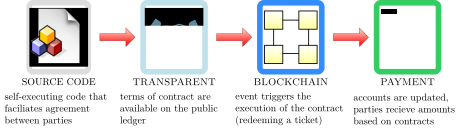
\includegraphics[width=1\linewidth]{smartContractsExp.pdf}
		\caption{Illustrating how a smart contract works}
		\label{fig:smartContracts}
	\end{figure}
\end{warpprint}

\begin{warpHTML}
	\begin{figure}[ht]
		\centering
		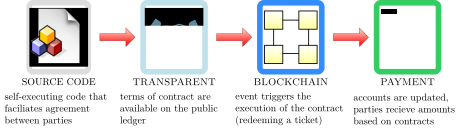
\includegraphics[width=1\linewidth]{smartContractsExp.svg}
		\caption{Illustrating how a smart contract works}
		\label{fig:smartContracts}
	\end{figure}
\end{warpHTML}

		In addition, irreversible and immutable transactions are a disadvantage that hackers can exploit. For example, an amateur coder killed the contract that allowed users to transfer Ether for the Parity \gls{Ethereum} Wallet, rendering 150 to 300 million dollars completely useless \cite{funnyJoke:Online}. Scrutinizing smart contracts and reducing bugs in production code is essential. An example of smart contract is available in Appendix A% \ref{lst:label}.
		
		% Rewrite here.
		The desirable properties of a \gls{blockchain} such as integrity and immutability of data, e.g., transactions and
		smart contracts, require an active mining pool. In a proof of work consensus (POW) mechanism,  miners need to invest energy and resources,
		i.e. computational power, to participate in the consensus process and prevent tampering blocks. Additionally, miners are incentivized to run nodes that verify transactions through bitcoin or ether. %The investment must incentive miners to verify transactions and/or run nodes.%This investment has to be incentivized to prevent miners from not participating.
	
\subsection{Representation of Digital Assets on the Blockchain}

\paragraph{ERC20 Token Standard}

The ERC20 token standard allows any tokens on Ethereum to be re-used by other applications: from wallets to decentralized exchanges. This is the most commonly used token on the Ethereum network at the moment.


\paragraph{ERC721 Token Standard}

Non-fungible tokens
The following standard allows for the implementation of a standard API for NFTs within smart contracts. This standard provides basic functionality to track and transfer NFTs.

We considered use cases of NFTs being owned and transacted by individuals as well as consignment to third party brokers/wallets/auctioneers ("operators"). NFTs can represent ownership over digital or physical assets. We considered a diverse universe of assets, and we know you will dream up many more:

Physical property — houses, unique artwork
Virtual collectables — unique pictures of kittens, collectable cards
"Negative value" assets — loans, burdens and other responsibilities

\paragraph{Other Smart Contracts}
Other contracts in the Harvest system, such as the storefront contract allow creation of reward tokens (ERC721s), however, since deploying ERC721s is gas intensive, a separate reward deployer contract is used and transfers ownership to the storefront. As shown in Figure xxx this averages out the deployment costs among other contracts.

\begin{figure}[H]
\centering
\includegraphics[width=1\linewidth]{Images/harvestArchitecture}
\caption{Architecture for smart contracts and front-end for harvest application}
\label{fig:harvestarchitecture}
\end{figure}

 Although determining the digital value of assets is challenging, the ability for a users to trade assets between themselves is essential for a decentralized marketplace. Implementation of a exchanger contract to buy/sell rewards and currencies are outside the scope of a proof of concept application.
%Participating music businesses will create a catalogue of valuable, real world offerings for the return of tokens from artists to the music business. Examples of products in this catalogue may include: studio recording sessions, record pressing, touring related costs, merchandise, and other goods and services. Music businesses will be encouraged to leverage existing business relationships to populate the catalogue of offerings. A music business offering this service may directly purchase rewards supply from vendors or work out rewards discounts that will be attractive to artists. 

%Music businesses who implement this tool will be differentiated from other distributors and rights managers. By adding an additional compensation and value to the way they compensate artists for plays, they will be able to create more loyalty and become even more attractive to potential artists. Every artist will benefit from the participation of previous artists as the economy of the MEC Rewards Program token grows. 


%	\end{minipage}
%%% New discussion
%%%%%%%%%%%%%%%%%%%%%%%%%%%%%%%%%%%%%%%%%%%%%%%%
%%%%%%% DISCUSSION %%%%%%%%%%%%%%%%%%%%%%%%%%%%%%
%%%%%%%%%%%%%%%%%%%%%%%%%%%%%%%%%%%%%%%%%%%%%%%%
\newpage
\section{Discussion}
 	The tools used in the harvest application are, a firefox/chrome plugin, metamask for connecting to the ethereum blockchain and testnets, the most popular framework for smart contract development truffle, and drizzle, which manages contract state.
		\subsection{Decentralized Applications}
		
		% Talk about drizzle metamask and truffle
		
		Decentralized systems are inherently more reliable, currently face scalability issues, and are trustless systems \cite{bitcoinWhitePaper:Online,ethereumWhitePaper:Online}. Fulfillment of smart contracts is limited due to off-chain information, logistical challenges in obtaining impartial or truthful inputs from stakeholders, and verification of transaction completion involving real-world assets. This suggests effectiveness of smart contracts is currently limited to digital assets rather than for physical assets.  In addition, translating legal-binding contracts to code is challenging because the majority of programmers lack a legal background.
		
		\begin{figure}[H]
		\centering
		\includegraphics[width=0.7\linewidth]{DappVApp}
		\caption{Decentralized structure vs Centralized Structure}
		\label{fig:dappvapp}
		\end{figure}
		
		Despite shortcomings that involve transactional steps that are computational impossible to verify (package is delivered), performance of smart contracts is superior as transactions are tamper-proof.
		Additionally, reduction of ambiguity from usage of smart contracts is highly probable because only one interpretation is possible. Coding errors or bugs exist in every non-trivial application, therefore transactions through smart contracts intrinsically carry some risk. This implies protocols and prior real-world agreements are necessary to migrate risk when executing smart contracts. Furthermore, increased precision and detail for transactional inputs and outputs required for creating smart contracts would benefit all parties. 
		
% \subsection{Functionality of Harvest}

 % Talk about token trading, creating new ERC721s
 	
 \subsection{Trading digital currency for rewards}
 \begin{algorithm}[ht]
   \caption{My first algorithm}\label{alg:algorithm1}
   \begin{algorithmic}[1]
     \Require
       \Statex If there are multiple lines here, line's number will be wrong.
       \Statex This error doesn't happen in package \verb|algorithmic|.
     \Ensure
       \Statex If I write \verb|\\| here, line's number will be wrong too.
     \Statex
     \If{$i = 1 \to n$} \Comment{This line's number should be 1}
       \State ${\textit{HU}}_{i} \gets {\textit{NGU}}_{i} + {HU}_{i}$ \Comment{Comment}
     \EndIf
   \end{algorithmic}
 \end{algorithm}
 
 
 % Creating new rewards in storefront 
 
 
  \begin{algorithm}[ht]
    \caption{Reward Creation}\label{alg:algorithm2}
    \begin{algorithmic}[1]
      \Require
        \Statex If there are multiple lines here, line's number will be wrong.
        \Statex This error doesn't happen in package \verb|algorithmic|.
      \Ensure
        \Statex If I write \verb|\\| here, line's number will be wrong too.
      \Statex
      \If{$i = 1 \to n$} \Comment{This line's number should be 1}
        \State ${\textit{HU}}_{i} \gets {\textit{NGU}}_{i} + {HU}_{i}$ \Comment{Comment}
      \EndIf
    \end{algorithmic}
  \end{algorithm}
 % Convert sequence diagram to state diagram showing how contracts are updated.
 % Include sequence diagram, or updated sequence diagram
\begin{figure}
\centering
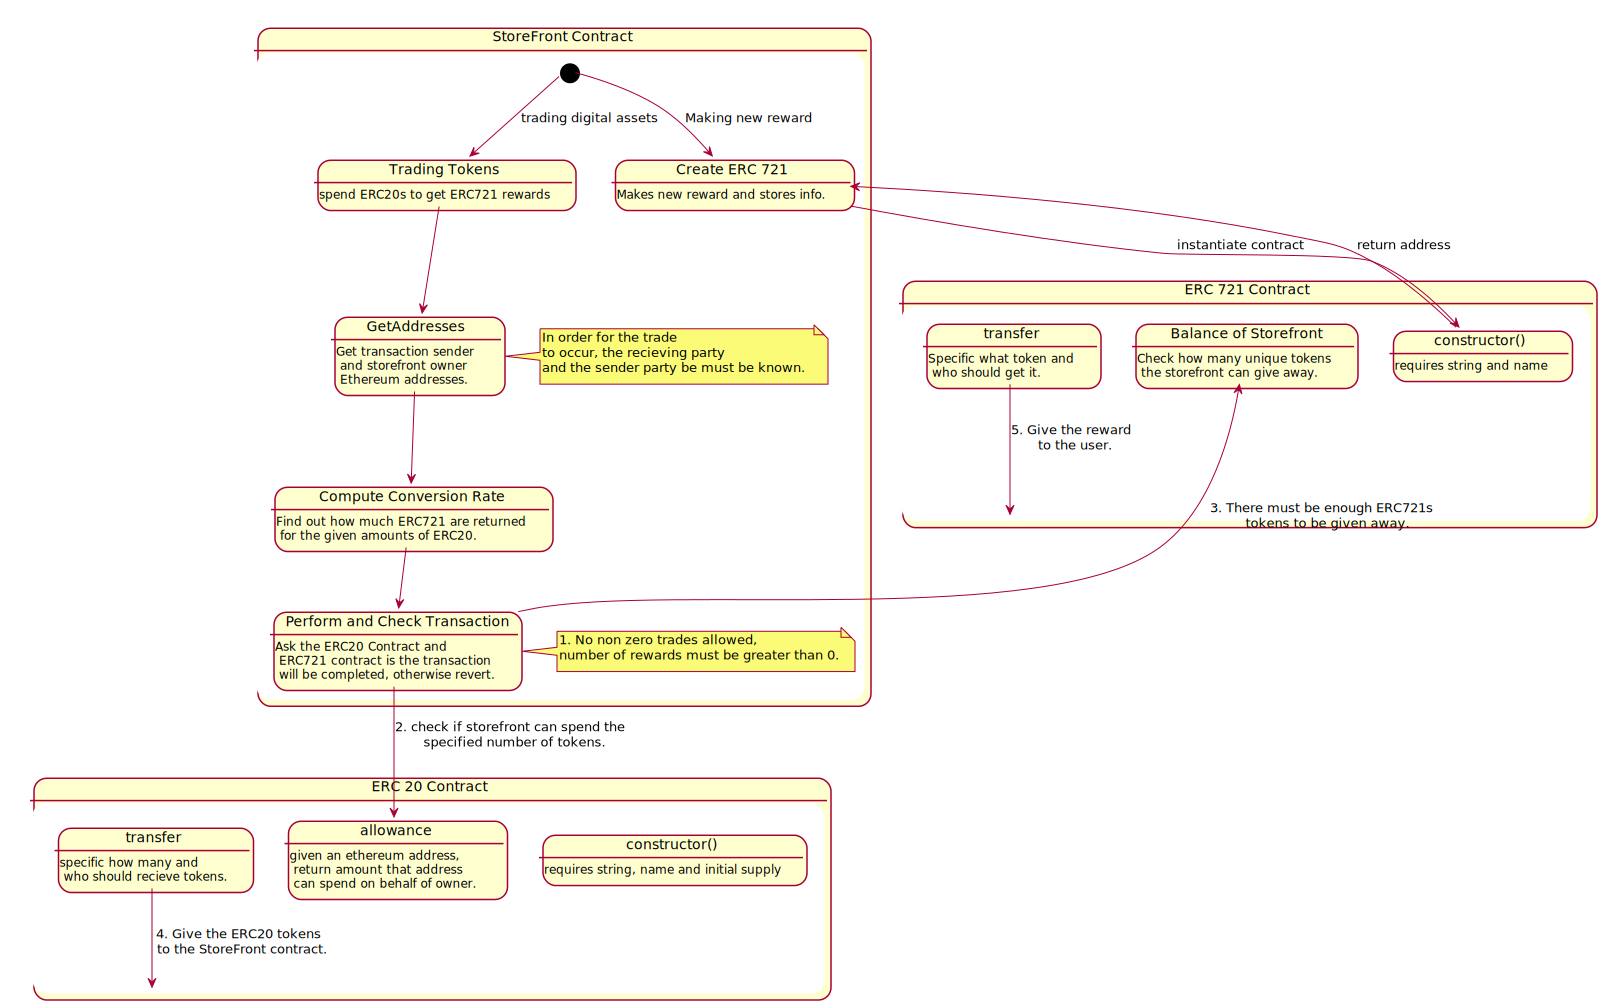
\includegraphics[width=1\linewidth]{StateDiagramENGR003}
\caption{State Diagram when a User wants to trade tokens}
\label{fig:statediagramengr003}
\end{figure}
 \subsection{Optimization of smart contracts}
 
 \paragraph{Limitations of Smart Contracts}
 % 24kb limit of data, 32 kb limit per transaction.
%	
\section{Discussion}
 Oftentimes, tacit information is trapped within emails, but using \gls{JIRA} and \gls{Confluence} together will capture this information forever. In addition, \gls{Confluence} and \gls{JIRA} have permissions to give flexibility to decide who can view and edit content.
 \subsection{JIRA}
Before JIRA Microsoft SharePoint, a document management system was used to “store, organize, share, and access information” \cite{sharepoint:Online}. An issue in JIRA is used to create, track and resolve reported client issues. MOTI IMB employees use JIRA on a daily basis, so an “issue could represent a software bug, a project task, a helpdesk ticket, etc.” \cite{issueDefinition:Online}.  \\

 JIRA is highly customizable, organized by projects, components, versions and labels. The most flexible way to search for issues is by constructing JQL (JIRA Query Languages) filters that use issue fields, operators, values and keywords and return specified JIRA issues. JIRA has spilt into 3 different standalone products JIRA Core, JIRA software, and JIRA Service Desk. Designed for managing projects and tasks, JIRA Core keeps team organized. JIRA Software allows for Agile boards and integrates with software development tools.  JIRA Service Desk is IT service desk and customer service software. JIRA incorporates time tracking, reporting features and is enhanced by installing add-ons such as ScriptRunner and Tempo Timesheets. Despite regular use of JIRA at MOTI IMB, its extensive functionality and plethora of features will confuse newcomers. 
 
 \subsubsection{Overview}
 Although JIRA originated as a software tool geared towards developers, it has evolved to address the needs of the non-technical users. \gls{JIRA} can track issues, display information on a dashboard and manage \gls{agile} projects by using \gls{kanban} or \gls{scrum} Boards which are designed to manage software projects. JIRA permissions are setting that limit what users can see and do. JIRA’s permission scheme includes editing issues, creating issues, commenting, assigning issues, etc. \cite{PermissionsOverview:Online}. Generally, users are added to an JIRA project, begin searching for issues, close \gls{issue} and repeat. 
  \subsubsection{Issues}
  An \gls{issue} contains multiple fields including type, priority, component, status, resolution, description assignee and reporter. It contains information indicating the urgency and current status of the issue. Some of the options available for issue status field include new, to-do, in progress, hold, and closed. Issue priorities vary from trivial to blocker. Classifying issues correctly is essential for users to document their work and reference in the future. Issues can have subtasks, be duplicated or be related to other existing issues. Watching an issue notified the user when the issue is commented, status changed, closed, or updated.
  \begin{figure}[H]
  	\includegraphics[width=1\linewidth]{cloud.jpg}
  	\caption{Clouds}
  \end{figure}
 \noindent When the status of an issue is changed or closed the reporter will receive an email update. Time tracking in \gls{JIRA} is accomplished by creating a work log, entering time spent, giving a reasonable remaining estimate and description of work done. Oftentimes, issues are reassigned to assignees better suited to complete the task. Attachments can be added to the issue to better describe work that needs to be done. Previously at IMB, for each application a Microsoft \gls{sharepoint} site would be created, and issue tracking was managed by creating list items. Even though this worked for small groups, providing access to each individual SharePoint site was cumbersome and time-consuming for everybody. A single system that contains issues for all projects benefits all users and has become essential to day-to-day operations. \\ 
 
 \noindent Issues in JIRA can be imported or exported to and from xls files, which allows the user to reuse content from fabricated in other applications. Overall, JIRA issues can represent anything ranging from software bugs, to an access request and used for project management.
 
 \subsubsection{Dashboards}
 JIRA dashboards contains information boxes known as gadgets that can display dynamic data about a JIRA filter or project. Gadgets let you customize the information that appears on dashboards. Configuring dashboards allows different kinds of information to be displayed.  Most of these gadgets require JIRA filters to feed information into it. Dashboards can display filter results, issue statistics, pie charts grouped by a specified issue field such as created, assignee, status, and priority. Add-ons for JIRA should as Zephyr (used for test management) and Tempo Timesheets (creates timesheets for JIRA issues) are packaged with dashboard gadgets containing additional information specific to that add on. An example is the user timesheet add-on from tempo which displays a timesheet for a specific period of time.  \\ 
 \begin{figure}[H]
 	\includegraphics[width=1\linewidth]{data1.jpg}
 	\caption{People}
 \end{figure}

At this time, dashboard usage is inconsistent, and undergoing further investigation. Ideally, every project and every team would have a JIRA dashboard, customized to suit their individual needs.  

Also, \gls{JIRA} has adaptable \gls{kanban} and \gls{scrum} boards to track issue backlogs. These boards can be displayed on a JIRA dashboard. Creating a meaningful dashboards faces several obstacles including understanding of the JIRA specific query language, \gls{jql}, knowledge of which dashboard gadget is suitable and a steep learning curve.  \\

Developing an informative \gls{JIRA} dashboard entails consulting with the end users, multiple iterations and producing JIRA filters.

 \begin{figure}[H]
	\includegraphics[width=1\linewidth]{datavisual.png}
	\caption{Visuallizing Data}
 \end{figure}

Dashboards are the best method to visually reporting on ongoing and completed issues in \gls{JIRA}.

\subsubsection{Agile Projects in JIRA}
Agile software development is used by the PEOPLE to produce software that better suits the needs of customers. 
In \gls{agile}, requirements and solutions develop through frequent conversations with stakeholders as software is developed through collaboration. Two kinds of agile boards are available in JIRA Agile, Kanban and Scrum. Each of these boards are designed to follow their specific agile methodology. Adding the fix version field to an issue will assign it to a particular release. All released and unreleased versions can be viewed within the project sidebar in JIRA. JIRA software provides tools specifically for any agile project management which include boards, releases and dashboard gadgets (burndown charts, velocity charts and more).

\begin{figure}[H]
	\includegraphics[width=1\linewidth]{q.jpg}
	\caption{Typical Pictures}
\end{figure}

\begin{table}
	\caption{Time log for ELEC 360 --- Assignment 2}
	\begin{tabular}{c c c c c}
		Week of Oct 8 &                 Week of Oct 15 &                      Week of Oct 22 &                                    Week of Nov 5 &                             Week of Nov 12 \\
		5 hours Prepared for ELEC 360 Lab and completed it &  2 hours working on lab report &  3 hours spent on preparing for lab &  3 hours doing the prelab and and lab experiment &  2 hours working on lab report \\
		3 hours of studying for quizzes &  3 hours studying for midterm &  2 hours studying midterm solutions &  2 hours reviewing for quizzes &  5 hours solving question for assignment 2 \\
		1 hour creating notes &  2 hours preparing for midterm &  2 hours preparing for quizzes &  3 hours solving questions of assignment 2 &  1 hour studying for quizzes \\
	\end{tabular}
\end{table}

Altogether, JIRA is well-suited for \gls{agile} project management with boards, versioning and dashboard gadgets.  

\subsubsection{Add-ons}
JIRA add-ons provide additional functionality to JIRA including increased customization and features. 

Adaptavist ScriptRunner provides custom workflows, custom JQL and executes scripts that interact with JIRA. Some notable features include custom automatic emails triggered when an issue transitions into a particular state, enhanced JIRA filters (i.e. searching for issues attachments) and adding additional fields for JIRA issues. This add-on provides a simple way to script in JIRA. \\ 

\noindent Tempo timesheets enhances time tracking and reporting features while faultlessly integrating with JIRA. It helps teams and managers track time, be efficient and used for forecasting. This add-on is useful because it allows JIRA users to accurate track their time spent on issues, projects and make strategic decisions based on this info. \\
The tempo time tracker runs within JIRA and is the best way track time.

\begin{figure}[H]
	\centering
	\includegraphics[width=0.4\textwidth,keepaspectratio]{final.jpg}
	\caption{Final Pictures}
\end{figure}

A user timesheet contains information about hours worked, planned, and required for the week. It organizes issues automatically organizes issues by project and component.

\begin{figure}[H]
	\centering
	\includegraphics[width=1\textwidth,keepaspectratio]{n.jpg}
	\caption{Cool Looking USBs.}
\end{figure}

\subsubsection{Limitations}
JIRA can be extremely slow at times which may be caused by running out of memory, and a large JIRA instance \cite{issues:Online}. Extensive functionality such as time tracking, \gls{agile} boards, dashboards and user timesheets are underutilised because users unaccustomed to JIRA. Additionally, a lack of tutorials or instructions are how to use JIRA compound the difficult of learning how to use \gls{JIRA}. 

\subsection {Confluence}
\gls{Confluence} is team-based collaboration software developed by Atlassian used at the ORGANIZATION to document projects and work in conjunction with \gls{JIRA}. Confluence works by It organizes content by labels, can embed videos on pages and is highly customizable. The aim of Confluence is to become the tool for organizing, discussing, and doing work. Assigning tasks, recording meeting notes and sharing documents are some of the features of Confluence.
\subsubsection{Overview}
Confluence keeps page and file versions to track every version of documents. Despite numerous free wiki-software available on the web, Confluence has page hierarchy (page trees), transparency when creating content and clean user interface which make it suitable for documentation.
\subsubsection{Spaces}
Everything in Confluence is organized in spaces, which are a collection of related pages. Pages are the documents in which the team will create, edit, and discuss work. Confluence Spaces are organized by categories (i.e., critical non-critical, documentation and software-project). Spaces can be customized to fit the need of each team. For example uses of Confluence include knowledge bases, technical documentation and organizing content \cite{confluence:Online}.
\subsubsection{Pages}
In a Confluence page, content is created, collected, and accessed in one place.

\begin{figure}[H]
	\centering
	\includegraphics[width=0.8\textwidth,keepaspectratio]{l.jpg}
	\caption{Creating Life}
\end{figure}

\noindent \gls{Confluence} pages contain text, images, videos and uses macros that add extra functionality or include dynamic content. Macros can create charts, incorporate existing Microsoft documents (Word, Excel, PowerPoint) and reuse content on Confluence pages. Existing templates in Confluence serve as an excellent starting point for users to start creating documentation for Confluence. Customizing page and space templates is an essential feature to save time and reuse content.

\subsubsection{Embedding Content}
Attachments are useful for sharing existing content saved in a different file format. 
\begin{figure}[H]
	\centering
	\includegraphics[width=0.5\textwidth,keepaspectratio]{good.jpg}
	\caption{Good Picture}
\end{figure} 
When word documents imported into Confluence, that document's content is copied onto one or more Confluence pages. Additionally, images and videos from the web can be embedded into a Confluence Page. Sharing links is convenient and helps users find information.

\subsubsection{Limitations}
Confluence is designed for documentation, used by large organizations including NASA \cite{NASA:Online}, yet documenting legacy and current projects in Confluence is not occurring at this moment. Currently, use of Confluence is limited to few internal users, so education about this software and its functionality lacking. Certain files types such as mpp (Microsoft Project) and vsd (Microsoft Visio) cannot be embedded within a Confluence Page, but can be uploaded as a file.  Creating structured space templates and pages will allow content to be streamlined. Confluence functionality can be extending by downloading add-on in the Atlassian marketplace. For example, tables in Confluence are rudimentary, consisting only of ascending/descending sorting, however, a few add-ons for Confluence address this problem.

\subsection{JIRA and Confluence Integration}
Much like how Microsoft Office Products integrate well together, JIRA and Confluence are better together. When \gls{Confluence} and JIRA sites are connected JIRA issues can be created, viewed and more from within Confluence. Also, connecting JIRA with Confluence allows pie charts, created vs resolved chart and filter results etc.  Essentially, existing information stored in JIRA can be reported in Confluence by the JIRA issues macro or the JIRA charts macro \cite{JAC:Online}.

\noindent Another benefit from connecting JIRA to \gls{Confluence} is delegated user management to \gls{JIRA}, so all users can be managed in a single location. Whenever a link is created to a JIRA issue in Confluence, or link to a Confluence page from a JIRA application, the JIRA Links button appears at the top of the Confluence page. This makes it very simple to jump from JIRA straight into Confluence and vice-versa.
\begin{figure}[H]
	\centering
	\includegraphics[width=0.5\textwidth,keepaspectratio]{goddata.jpg}
	\caption{Good Looking Report}
\end{figure} 
\noindent The tight integration between Confluence and JIRA results in related issues can be accessed directly from the Confluence page with their current status.

\begin{figure}
\centering
\includegraphics[width=1\linewidth]{smartContractCreation}
\caption{Lifecycle of Smart Contract Creation \cite{Sillaber2017}}
\label{fig:smartcontractcreation}
\end{figure}

As shown in figure \ref{fig:smartcontractcreation} multiple parties are required to create comprenhensive smart contract, input from legal professions and negotiations are required.

\newpage 
\section{Conclusion}

Decentralized systems are inherently more reliable, resilient against brute force attacks, and are more transparent \cite{bitcoinWhitePaper:Online,ethereumWhitePaper:Online}. Fulfillment of smart contracts is limited due to off-chain information, logistical challenging obtaining impartial or truthful inputs from stakeholders, and verification of transaction completion involving real-world assets. This suggests effectiveness of smart contracts is currently limited to digital assets rather than for physical assets.  In addition, translating legal-binding contracts to code is challenging because the majority of programmers lack a legal background.

\begin{figure}[H]
\centering
\includegraphics[width=0.7\linewidth]{Diagrams/DappVApp}
\caption{Decentralized structure vs Centralized Structure}
\label{fig:dappvapp}
\end{figure}

Despite shortcomings that involve transactional steps that are computational impossible to verify (package is delivered), performance of smart contracts is superior as transactions are tamper-proof.
Additionally, reduction of ambiguity from usage of smart contracts is highly probable because only one interpretation is possible. Coding errors or bugs exist in every non-trivial application, therefore transactions through smart contracts intrinsically carry some risk. This implies protocols and prior real-world agreements are necessary to migrate risk when executing smart contracts. Furthermore, increased precision and detail for transactional inputs and outputs required for creating smart contracts would benefit all parties. 

As shown in Figure \ref{security:fig2} only computers with significant high processing power  (quantum computers) can decrypt a 256 bit ethereum key cost-effectively. This indicates trying to hacking private keys is not a worthwhile venture.
Overall, smart contracts in conjunction with blockchain technologies allow for users to have a unique digital presence, securely transfer ownership of assets and avoid key shortcomings of centralized IT systems.

\newpage
%Despite Even though immutable and irreversible transactions are advantageous, criminals leverage cryptocurrencies for illegal transfer of funds. %This implies the ability to undo fraudulent or criminal activity is extremely important, but reversible transactions is an anti-pattern. %For example EOS, a centralized blockchain platform, was criticized for freezing accounts without due process and community backing. \cite{EOS:Online}. In addition, centralized systems require users to trust vendors and oftentimes personal data usage lacks transparency. Currently, research into blockchain technologies are actively researched that can disrupt existing industries including finance, real-estate and supply chains. \hfill \break
% 

%Deployment of a smart contract is inexpensive, however, development and maintenance costs for blockchain applications can be costly. This implies that transaction expenses decrease significantly, but running a blockchain node, ensuring high quality code for smart contracts is challenging and expensive. Decentralized applications are transparent because information is available in the publicly ledger and parties participating in a transaction cannot alter it. Overcomplicated code and bugs in smart contracts are severely detrimental because of malicious transactions by scammers or hackers. \hfill \break


%Smart contract reduce complexity of transactions allowing buyers to directly interact with sellers. This illustrates how useful smart contracts are, but lack of legislation for blockchain technologies, consortiums unwilling to adopt decentralized applications (may prefer private blockchains), and ability for hackers to exploit bugs suggest transactions governed by code is decades away. Solutions to existing problems in blockchain technologies such as latency, immutable transactions and widespread acceptance by consortiums are addressed through innovations such as sidechains, centralized blockchain platforms like EOS and private blockchains infrastructure. \hfill \break

\newpage
 \section{Recommendations}
 
 
  
Obviously continued researching into \gls{blockchain} technologies is necessary as innovations such as permissioned blockchains such as \gls{HyperLedger Composer} and \gls{side chains} continue to address some shortcomings of blockchain. In trustless systems tampering or modification of transactional history is extremely difficult. This suggests that smart contracts can greatly improve transactions, however, issues including scalability, reversing fraudulent activity and reduction of contract deployment hinder mass adoption.

All computer programs have bugs, by limiting complexity of smart contracts,  using reliable standards highly audited packages, and using software security analyze tools risk can be greatly reduced. Continuing to monitor technology innovations such ever-increasing computational power is important to ensure cracking private keys remain uneconomical see Figure \ref{security:fig2}.

Provided a deterministic set of inputs and outputs, with computational verifiable conditions, using smart contracts is beneficial.
Increasing awareness about \gls{blockchain} technologies, so that the average person understands the limitations of smart contracts and in what situations they can be useful.

\newpage
%%%%%%%%%%%%%%%%%%%%%%%%%%%%%%%%%%%%%%%%%%%%%%
%%%% END Main Content %%%%%%%%%%%%%%%%%%%
%%%%%%%%%%%%%%%%%%%%%%%%%%%%%%%%%%%%%%%%%%%%%%

%%%%%%%%%%%%%%%%%%%%%%%%%%%%%%%%%%%%%%%%%%%%%%
%%% BACK MATTER, printing References %%%%%%%%%
%%%%%%%%%%%%%%%%%%%%%%%%%%%%%%%%%%%%%%%%%%%%%%
\renewcommand\bibname{References} % Change bibliography to references

% nocite prints all references even if they were not used
% \nocite{*}
\newpage 
 \printbibliography
 
\linespread{1}

\newpage 
\begin{appendices}
\section{Token Standards}
%\lstinputlisting[
%language   = C,
%basicstyle = \ttfamily,
%style		= default,
%%frame      = single,
%caption    = {Caesar Cipher for CSC 111},]
%{Code/cipher.c}
\begin{lstlisting}[language=Solidity,caption=ERC20 Token Standard Interface]
pragma solidity ^0.4.20;
contract ERC20Interface {
    function totalSupply() public constant returns (uint);
    function balanceOf(address tokenOwner) public constant returns (uint balance);
    function allowance(address tokenOwner, address spender) public constant returns (uint remaining);
    function transfer(address to, uint tokens) public returns (bool success);
    function approve(address spender, uint tokens) public returns (bool success);
    function transferFrom(address from, address to, uint tokens) public returns (bool success);

    event Transfer(address indexed from, address indexed to, uint tokens);
    event Approval(address indexed tokenOwner, address indexed spender, uint tokens);
}
\end{lstlisting}

\begin{lstlisting}[language=Solidity, caption=ERC721 Token Standard Interface]
pragma solidity ^0.4.20;

contract ERC721 {
    event Transfer(address indexed _from, address indexed _to, uint256 indexed _tokenId);
    event Approval(address indexed _owner, address indexed _approved, uint256 indexed _tokenId);
    event ApprovalForAll(address indexed _owner, address indexed _operator, bool _approved);
    function balanceOf(address _owner) external view returns (uint256);
    function ownerOf(uint256 _tokenId) external view returns (address);
    function safeTransferFrom(address _from, address _to, uint256 _tokenId, bytes data) external payable;
    function safeTransferFrom(address _from, address _to, uint256 _tokenId) external payable;
    function transferFrom(address _from, address _to, uint256 _tokenId) external payable;
    function approve(address _approved, uint256 _tokenId) external payable;
    function setApprovalForAll(address _operator, bool _approved) external;
    function getApproved(uint256 _tokenId) external view returns (address);
    function isApprovedForAll(address _owner, address _operator) external view returns (bool);
}

\end{lstlisting}
\end{appendices}
\end{document}

%%%%%%%%%%%%%%%%
COMMON COMMANDS:
%%%%%%%%%%%%%%%%
% IMAGES
\begin{figure}[H]
	\begin{center}
		\includegraphics[width=0.6\textwidth]{RTL_SCHEM.png}
	\end{center}
	\caption{A screenshot of the RTL Schematics produced from the Verilog code.}
	\label{RTL}
\end{figure}

% SUBFIGURES IMAGES
\begin{figure}[H]
	\centering
	\subfloat[LED4 Period]{\label{fig:Per4}\includegraphics[width=0.4\textwidth]{period_led4.png}} \\                
	\subfloat[LED5 Period]{\label{fig:Per5}\includegraphics[width=0.4\textwidth]{period_led5.png}}
	\subfloat[LED6 Period]{\label{fig:Per6}\includegraphics[width=0.4\textwidth]{period_led6.png}}
	\caption{Period of LED blink rate captured by osciliscope.}
	\label{fig:oscil}
\end{figure}

% CITATIONS
\cite{CitationName}

% GLOSSARY ENTRY
\newglossaryentry{api}
{
	name={API},
	description={An Application Programming Interface (API) is a particular set
		of rules and specifications that a software program can follow to access and make use of the services and resources provided by another particular software program that implements that API},
	first={Application Programming Interface (API)},
	long={Application Programming Interface}
}
% INSERT SOURCE CODE
\lstinputlisting[
language=SQL,
basicstyle = \ttfamily,
style=			Oracle,
%frame      = single,
caption    = {Sample SQL Query},]
{Code/Data.sql}

% FANCY TABLE
\begin{table}
	\begin{center}
	\begin{tabular}{@{} l *4c @{}}
		\toprule
		\multicolumn{1}{c}{Models}    & A  & B  & C  & D  \\ 
		\midrule
		Model $X$ & X1 & X2 & X3 & X4 \\ 
		Model $Y$ & Y1 & Y2 & Y3 & Y4 \\
		\bottomrule
	\end{tabular}
	\caption{Caption}
	\end{center}
\end{table}

% TEXT TABLE
\begin{table}
	\begin{center}
		\begin{tabular}{|l|c|c|l|}
			x & x & x & x \\ \hline
			x & x & x & x \\
			x & x & x & x \\ \hline
		\end{tabular}
		\caption{Caption}
		\label{label}
	\end{center}
\end{table}

% MATHMATICAL ENVIRONMENT
$ 8 = 2 \times 4 $

% CENTERED FORMULA
\[  \]

% NUMBERED EQUATION
\begin{equation}

\end{equation}

% ARRAY OF EQUATIONS (The splat supresses the numbering)
\begin{align*}

\end{align*}

% NUMBERED ARRAY OF EQUATIONS
\begin{align}

\end{align}

% ACCENTS
\dot{x} % dot
\ddot{x} % double dot
\bar{x} % bar
\tilde{x} % tilde
\vec{x} % vector
\hat{x} % hat
\acute{x} % acute
\grave{x} % grave
\breve{x} % breve
\check{x} % dot (cowboy hat)

% FONTS
\mathrm{text} % roman
\mathsf{text} % sans serif
\mathtt{text} % Typewriter
\mathbb{text} % Blackboard bold
\mathcal{text} % Caligraphy
\mathfrak{text} % Fraktur

\textbf{text} % bold
\textit{text} % italic
\textsl{text} % slanted
\textsc{text} % small caps
\texttt{text} % typewriter
\underline{text} % underline
\emph{text} % emphasized

\begin{tiny}text\end{tiny} % Tiny
\begin{scriptsize}text\end{scriptsize} % Script Size
\begin{footnotesize}text\end{footnotesize} % Footnote Size
\begin{small}text\end{small} % Small
\begin{normalsize}text\end{normalsize} % Normal Size
\begin{large}text\end{large} % Large
\begin{Large}text\end{Large} % Larger
\begin{LARGE}text\end{LARGE} % Very Large
\begin{huge}text\end{huge}   % Huge
\begin{Huge}text\end{Huge}   % Very Huge

%   \Gls{agile} software development uses repeatable brief cycles called 
%   \glspl{sprint} that focus on short-term deliverables.
\begin{figure}
	\caption{A picture323}
\end{figure}
\begin{table}[H]
	\begin{center}
		\begin{tabular}{cccc}
			\toprule 
			Nucleus & \textit{I} & Natural Abundance / \% & Larmor Frequency @ 7T \\
			\midrule
			\rowcolor{black!20} \textsuperscript{1}H & \sfrac{1}{2} & 99.98 & 298.0 \\
			\textsuperscript{2}H & 1 & 0.02 & 45.7 \\
			\rowcolor{black!20} \textsuperscript{12}C & 0 & 98.90 & - \\
			\textsuperscript{13}C & \sfrac{1}{2} & 1.10 & 74.9 \\
			\rowcolor{black!20} \textsuperscript{14}N & 1 & 99.60 & 21.5 \\
			\textsuperscript{15}N & \sfrac{1}{2} & 0.40 & 30.2 \\
			\rowcolor{black!20} \textsuperscript{16}O & 0 & 99.96 & - \\
			\textsuperscript{17}O & \sfrac{1}{2} & 0.04 & 40.4 \\
			\bottomrule
		\end{tabular}
		\caption{Numbers232323}
	\end{center}
\end{table}

%%% COMPLETE TABLE EXAMPLE %%%%
\newcommand{\head}[1]{\textnormal{\textbf{#1}}}
\newcommand{\normal}[1]{\multicolumn{1}{l}{#1}}
\begin{table}
	\centering
	\begin{tabular}{@{}l*2{>{\textbackslash\ttfamily}l}%
			l<{Example text}l@{}}
		\toprule[1.5pt]
		& \multicolumn{2}{c}{\head{Input}}
		& \multicolumn{2}{c}{\head{Output}}\\
		& \normal{\head{Command}} & \normal{\head{Declaration}}
		& \normal{\head{Single use}} & \head{Combined}\\
		\cmidrule(lr){2-3}\cmidrule(l){4-5}
		\multirow{3}{*}{Family} &  textrm & rmfamily & \rmfamily & \\
		& textsf & sffamily & \sffamily & \\
		& texttt & ttfamily & \ttfamily & \\
		\cmidrule(lr){2-3}\cmidrule(lr){4-4}
		\multirow{2}{1.1cm}{Weight} & textbf & bfseries & \bfseries
		& \multirow{2}{1.8cm}{\sffamily\bfseries Bold and sans-serif} \\
		& textmd & mdseries & \mdseries & \\
		\cmidrule(lr){2-3}\cmidrule(lr){4-4}
		\multirow{4}{*}{Shape} & textit & itshape & \itshape & \\
		& textsl & slshape & \slshape &
		\multirow{2}{1.8cm}{\sffamily\slshape Slanted and sans-serif}\\
		& textsc & scshape & \scshape & \\
		& textup & upshape & \upshape & \\
		\cmidrule(lr){2-3}\cmidrule(lr){4-4}
		Default & textnormal & normalfont & \normalfont & \\
		\bottomrule[1.5pt]
	\end{tabular}
	\caption{\LaTeX\ font selection}
\end{table}
%%%%    END TABLE EXAMPLE   %%%%%

%%%% TABLE EXAMPLE %%%%
\newcolumntype{Y}{>{\raggedleft\arraybackslash}X}

\tcbset{tab1/.style={fonttitle=\bfseries\large,fontupper=\normalsize\sffamily,
		colback=yellow!10!white,colframe=red!75!black,colbacktitle=orange!40!white,
		coltitle=black,center title,freelance,frame code={
			\foreach \n in {north east,north west,south east,south west}
			{\path [fill=red!75!black] (interior.\n) circle (3mm); };},}}

\tcbset{tab2/.style={enhanced,fonttitle=\bfseries,fontupper=\normalsize\sffamily,
		colback=yellow!10!white,colframe=red!50!black,colbacktitle=yellow!40!white,
		coltitle=black,center title}}
\begin{table}
	\begin{tcolorbox}[tabularx={X||Y|Y|Y|Y||Y},title=My table]
		Group & One & Two & Three & Four & Sum\\\hline\hline
		Red & 1000.00 & 2000.00 & 3000.00 & 4000.00 & 10000.00\\\hline
		Green & 2000.00 & 3000.00 & 4000.00 & 5000.00 & 14000.00\\\hline
		Blue & 3000.00 & 4000.00 & 5000.00 & 6000.00 & 18000.00\\\hline\hline
		Sum & 6000.00 & 9000.00 & 12000.00 & 15000.00 & 42000.00
	\end{tcolorbox}
	\caption{Another Great Table}
\end{table}
\begin{table}
	\begin{tcolorbox}[tab1, tabularx={X||Y|Y|Y|Y||Y}]
		Group & One & Two & Three & Four & Sum\\\hline\hline
		Red & 1000.00 & 2000.00 & 3000.00 & 4000.00 & 10000.00\\\hline
		Green & 2000.00 & 3000.00 & 4000.00 & 5000.00 & 14000.00\\\hline
		Blue & 3000.00 & 4000.00 & 5000.00 & 6000.00 & 18000.00\\\hline\hline
		Sum & 6000.00 & 9000.00 & 12000.00 & 15000.00 & 42000.00
	\end{tcolorbox}
	\caption{Great Table}
\end{table}
\begin{table}
	\begin{tcolorbox}[tab2, tabularx={X||Y|Y|Y|Y||Y},title=My table]
		Group & One & Two & Three & Four & Sum\\\hline\hline
		Red & 1000.00 & 2000.00 & 3000.00 & 4000.00 & 10000.00\\\hline
		Green & 2000.00 & 3000.00 & 4000.00 & 5000.00 & 14000.00\\\hline
		Blue & 3000.00 & 4000.00 & 5000.00 & 6000.00 & 18000.00\\\hline\hline
		Sum & 6000.00 & 9000.00 & 12000.00 & 15000.00 & 42000.00
	\end{tcolorbox}
	\caption{Good Table}
\end{table}
%%%% END TABLE EXAMPLE %%%%

%ANOTHER TABLE EXAMPLE
\setlist{nolistsep}
\definecolor{green}{HTML}{66FF66}
\definecolor{myGreen}{HTML}{009900}

%\renewcommand{\familydefault}{\sfdefault}


\begin{table}
	\begin{center}
		\begin{tabularx}{\textwidth}[t]{XX}
			\arrayrulecolor{green}\hline
			\textbf{\textcolor{myGreen}{Goal 1 Eradicate Extreme Poverty}} & \\
			\hline
			Target 1.A Halve, between 1990 and 2015, the proportion of the people whose income is less than \$1 a day. & 
			\begin{minipage}[t]{\linewidth}%
				\begin{itemize}
					\item[1.1] Proportion of population below \$1 purchasing power parity (PPP) a day$^a$
					\item[1.2] Poverty Gap ratio [incidence x depth of poverty]
					\item[1.3] Share of the poorest quintile in national consumption
				\end{itemize} 
			\end{minipage}\\
			
			\arrayrulecolor{black}\hline
			
			Target 1.B Achieve full and productive employment and decent work for all, including women and young people &
			\begin{minipage}[t]{\linewidth}%
				\begin{itemize}
					\item[1.4] Growth of GDP per person employed 
					\item[1.5] Employment to population ratio
					\item[1.6] Proportion of employed people living below \$1 (PP) a day
					\item[1.7] Proportion of own-account and contribution family workers in total employment
				\end{itemize} 
			\end{minipage}\\
			
			\hline
			
			Target 1.C Halve, between 1990 and 2015, the proportion of people who suffer from hunger &
			\begin{minipage}[t]{\linewidth}%
				\begin{itemize}
					\item[1.8] Prevalence of underweight children under five years of age
					\item[1.9] Proportion of population below minimum level of dietary energy consumption
				\end{itemize}
			\end{minipage}\\
			
			\arrayrulecolor{green}\hline
			\textbf{\textcolor{myGreen}{Goal 2 Achieve universal primary education}} \\
			\hline
			
			Target 2.A Ensure that by 2015 children everywhere, boy and girls alike, will be able to complete a full course of primary schooling. &
			\begin{minipage}[t]{\linewidth}%
				\begin{itemize}
					\item[2.1] Net enrollment ratio in primary education
					\item[2.2] Proportion of pupils starting grade 1 who reach last grade of primary education
					\item[2.3] Literacy rate of 15- to 24-year-olds, women and men
				\end{itemize}
			\end{minipage}\\
			
			\hline
			\multicolumn{2}{l}{%
				\textbf{\textcolor{myGreen}{Goal 3 Promote gender equality and empower women}}} \\
			\hline
			
			Target 3.A Eliminate gender disparity in primary and secondary education, preferably by 2005, and in all levels of education no later than 2015 &
			\begin{minipage}[t]{\linewidth}%
				\begin{itemize}
					\item[3.1] Ratios of girls to boys in primary, secondary and tertiary education
					\item[3.2] Share of women in wage employment in the non-agricultural sector.
				\end{itemize} 
			\end{minipage}
		\end{tabularx}
	\end{center}
	\caption{Great table to use}
\end{table}
% END ANOTHER TABLE EXAMPLE
\begin{figure}
	\caption{Another picture2323}
\end{figure}


\lstinputlisting[
language=SQL,
basicstyle = \ttfamily,
style=			Oracle,
caption    = {Sample SQL Query},]
{Code/Data.sql}	

\begin{table}
	\begin{center}
		\begin{tabular}{ |l|l|l| }
			\hline
			\multicolumn{3}{ |c| }{Team sheet} \\
			\hline
			Goalkeeper & GK & Paul Robinson \\ \hline
			\multirow{4}{*}{Defenders} & LB & Lucas Radebe \\
			& DC & Michael Duburry \\
			& DC & Dominic Matteo \\
			& RB & Didier Domi \\ \hline
			\multirow{3}{*}{Midfielders} & MC & David Batty \\
			& MC & Eirik Bakke \\
			& MC & Jody Morris \\ \hline
			Forward & FW & Jamie McMaster \\ \hline
			\multirow{2}{*}{Strikers} & ST & Alan Smith \\
			& ST & Mark Viduka \\
			\hline
		\end{tabular}
	\end{center}
	\caption{Table Title}
\end{table}

\begin{table} 
	\begin{center}
		\begin{tabular}{cccccccc} \toprule
			{$m$} & {$\Re\{\underline{\mathfrak{X}}(m)\}$} & {$-\Im\{\underline{\mathfrak{X}}(m)\}$} & {$\mathfrak{X}(m)$} & {$\frac{\mathfrak{X}(m)}{23}$} & {$A_m$} & {$\varphi(m)\ /\ ^{\circ}$} & {$\varphi_m\ /\ ^{\circ}$} \\ \midrule
			1  & 16.128 & +8.872 & 16.128 & 1.402 & 1.373 & -146.6 & -137.6 \\
			2  & 3.442  & -2.509 & 3.442  & 0.299 & 0.343 & 133.2  & 152.4  \\
			3  & 1.826  & -0.363 & 1.826  & 0.159 & 0.119 & 168.5  & -161.1 \\
			4  & 0.993  & -0.429 & 0.993  & 0.086 & 0.08  & 25.6   & 90     \\ \midrule
			5  & 1.29   & +0.099 & 1.29   & 0.112 & 0.097 & -175.6 & -114.7 \\
			6  & 0.483  & -0.183 & 0.483  & 0.042 & 0.063 & 22.3   & 122.5  \\
			7  & 0.766  & -0.475 & 0.766  & 0.067 & 0.039 & 141.6  & -122   \\
			8  & 0.624  & +0.365 & 0.624  & 0.054 & 0.04  & -35.7  & 90     \\ \midrule
			9  & 0.641  & -0.466 & 0.641  & 0.056 & 0.045 & 133.3  & -106.3 \\
			10 & 0.45   & +0.421 & 0.45   & 0.039 & 0.034 & -69.4  & 110.9  \\
			11 & 0.598  & -0.597 & 0.598  & 0.052 & 0.025 & 92.3   & -109.3 \\ \bottomrule
		\end{tabular}
	\end{center}
	\caption{Table Title}
\end{table}